\chapter{Éléments complémentaires}

\section{Périodicité, bords et phénomène de Gibbs}
\label{app:periodicite-bords-gibbs}

Dans ce mémoire, nous utilisons fréquemment la transformée de Fourier discrète et la convolution
circulaire. Ces outils reposent implicitement sur une hypothèse de périodisation du signal. Il est donc
utile de rappeler brièvement le lien entre périodicité, spectre de Fourier et effets de bord.

\begin{itemize}
    \item Si un signal est défini sur un domaine infini, par exemple sur $\mathbb{R}$, et qu'il n'est pas périodique,
    alors son contenu fréquentiel est décrit par un \emph{spectre continu}. On parle alors de transformée de Fourier.

    \item Si un signal est périodique, son contenu fréquentiel devient au contraire \emph{discret} :
    le signal se décompose en une somme de modes harmoniques de fréquences bien déterminées.
    On parle dans ce cas de série de Fourier.

    \item Enfin, dans le cas des signaux numériques de longueur finie, on utilise souvent une hypothèse de
    périodisation. Le signal est alors considéré comme périodiquement prolongé : ses deux extrémités sont
    artificiellement raccordées, comme si l'on enroulait la feuille sur laquelle il est tracé pour former une boucle.
\end{itemize}

Cette hypothèse est mathématiquement très utile, car elle permet d'utiliser la transformée de Fourier
discrète et de représenter certaines convolutions comme des convolutions circulaires. Elle peut cependant
introduire un artefact lorsque les bords du signal ne se raccordent pas naturellement. Si le bord droit ne rejoint pas le bord gauche avec une valeur
compatible, une discontinuité artificielle apparaît à la jonction.

Cette discontinuité est importante du point de vue de Fourier. En effet, une approximation par un nombre fini de modes de Fourier représente difficilement un saut
abrupt. Elle produit alors des oscillations parasites au voisinage de
la coupure. Ce comportement est connu sous le nom de phénomène de Gibbs~\cite{oppenheim2009discrete}.

\begin{figure}[H]
    \centering
    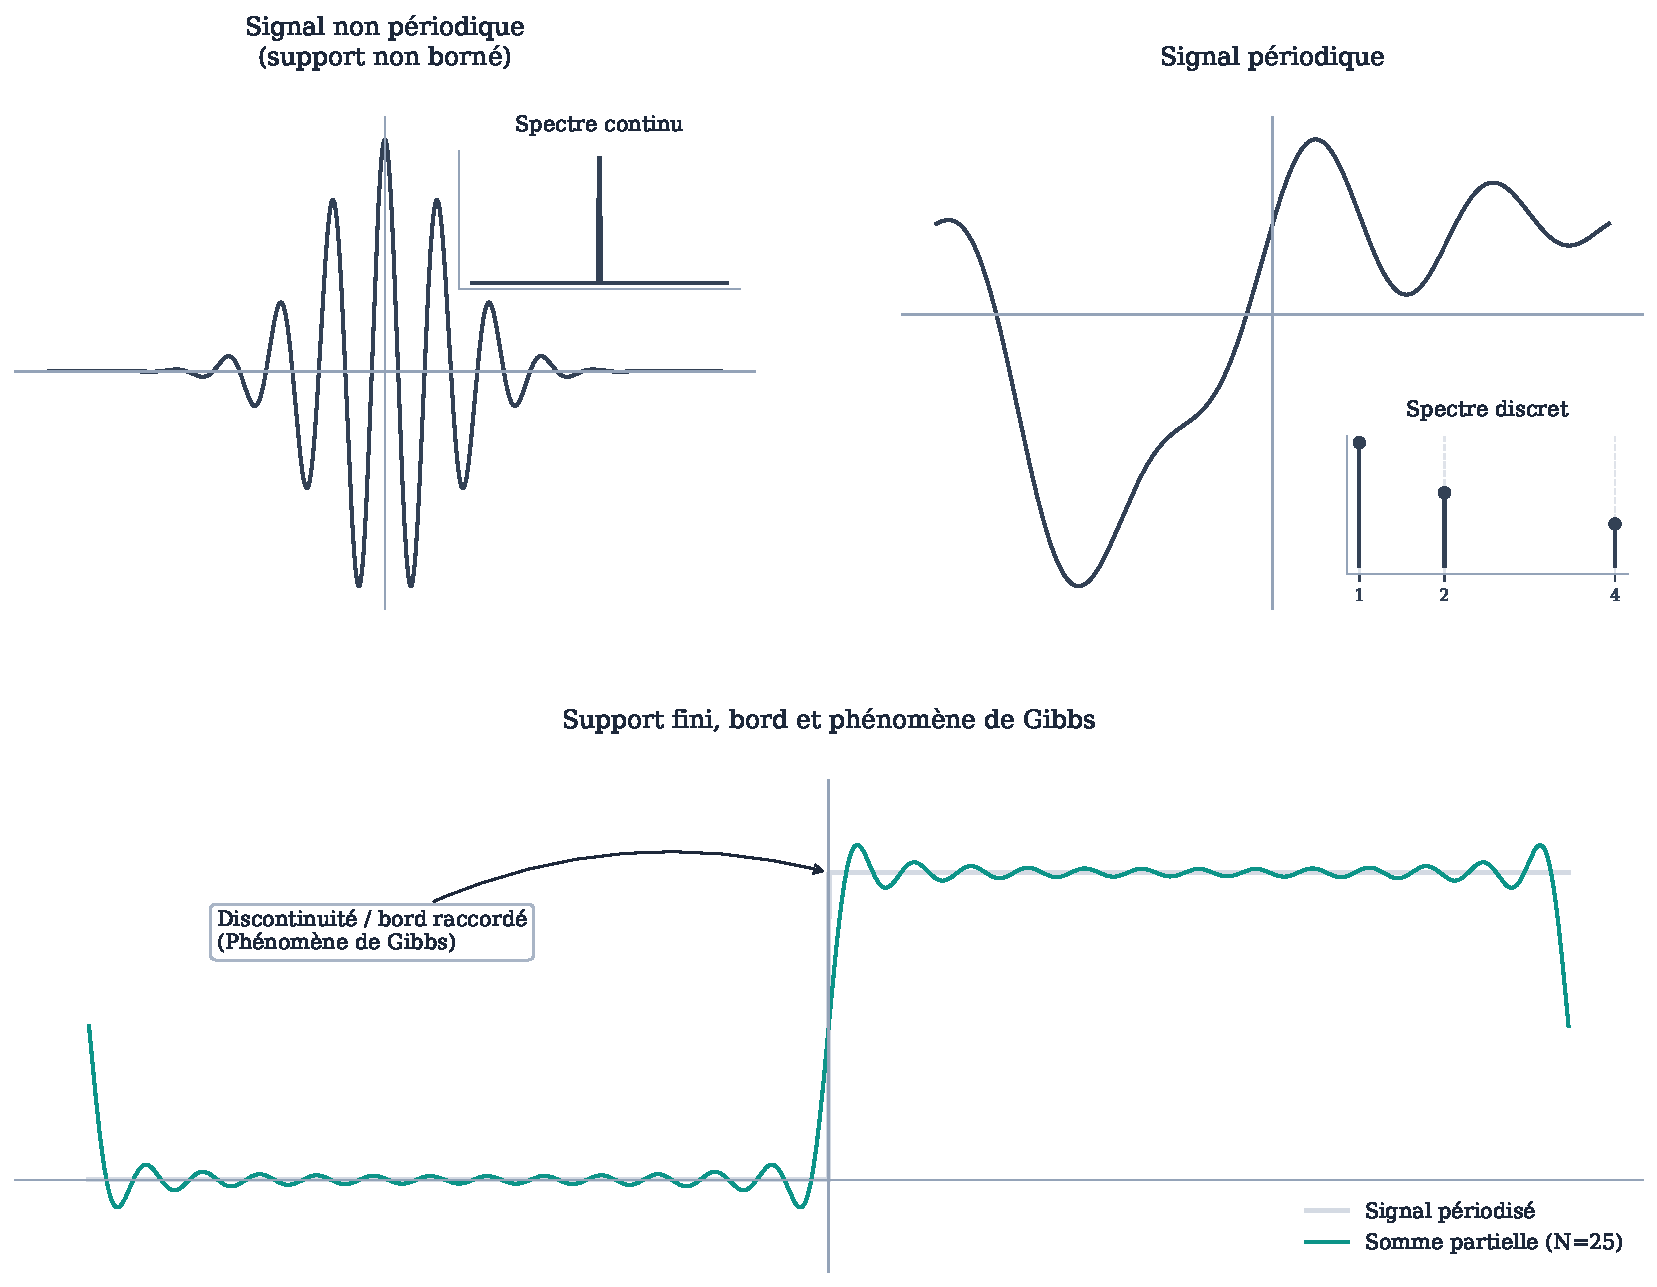
\includegraphics[width=0.8\textwidth]{figures/theory/fourier_periodicite_gibbs.pdf}
    \caption{À gauche : un signal non périodique défini sur un domaine infini possède un spectre continu.
    Au centre : un signal périodique possède un spectre discret constitué de raies harmoniques.
    À droite : un signal de support fini peut présenter une discontinuité artificielle lorsqu'il est périodisé.}
    \label{fig:gibbs}
\end{figure}

\section{Détail de la preuve de la structure BCCB}
\label{app:preuve_bccb}

On reprend ici le cas d'une convolution circulaire 2D mono-canal. L'objectif est de montrer,
pas à pas, pourquoi la matrice $M$ associée à cette convolution est circulante par blocs, 
et chacun de ses blocs est lui-même circulant.

\begin{proof}

On note $X\in\mathbb{C}^{N\times N}$ l'image d'entrée, $Y\in\mathbb{C}^{N\times N}$ l'image de
sortie, et $h\in\mathbb{C}^{N\times N}$ le filtre. On rappelle que dans le cadre circulaire, la convolution 2D s'écrit

$$\begin{aligned}
    Y[m,n] &= \sum_{a=0}^{N-1} \sum_{b=0}^{N-1} h[a,b] \, X[(m-a)\bmod N, \, (n-b)\bmod N] \\
           &= \sum_{a=0}^{N-1} \sum_{b=0}^{N-1} h[(m-a)\bmod N, \, (n-b)\bmod N] \, X[a, b].
\end{aligned}$$

Avec la vectorisation par colonnes, l'entrée $X[r,s]$ correspond à l'indice vectorisé
$r+Ns$, et la sortie $Y[m,n]$ correspond à l'indice vectorisé $m+Nn$. La matrice $M$ est définie
par
\[
    \operatorname{vec}(Y)=M\operatorname{vec}(X).
\]
Le coefficient de $M$ situé à la ligne $m+Nn$ et à la colonne $r+Ns$ indique donc comment le pixel
$X[r,s]$ contribue au pixel $Y[m,n]$.

D'après la formule de convolution 2D, cette contribution est donnée par
\[
    M_{m+Nn,\;r+Ns}
    =
    h[(m-r)\bmod N,\,(n-s)\bmod N].
\]
Cette formule est le point central de la preuve : le coefficient dépend seulement des décalages
circulaires entre les positions d'entrée et de sortie.

On découpe maintenant la matrice $M$ en $N\times N$ blocs, chacun de taille $N\times N$ :
\[
M =
\begin{pmatrix}
B_{0,0} & B_{0,1} & \cdots & B_{0,N-1} \\
B_{1,0} & B_{1,1} & \cdots & B_{1,N-1} \\
\vdots  & \vdots  & \ddots & \vdots \\
B_{N-1,0} & B_{N-1,1} & \cdots & B_{N-1,N-1}
\end{pmatrix}.
\]
Dans ce découpage, le bloc $B_{n,s}$ décrit l'effet de la colonne $s$ de l'image d'entrée sur la
colonne $n$ de l'image de sortie.

Les coefficients de ce bloc sont donc
\[
    (B_{n,s})_{m,r}
    =
    M_{m+Nn,\;r+Ns}
    =
    h[(m-r)\bmod N,\,(n-s)\bmod N].
\]

Fixons maintenant deux colonnes $n$ et $s$. Leur décalage circulaire est
\[
    \delta = (n-s)\bmod N.
\]
Avec cette notation, l'expression précédente devient
\[
    (B_{n,s})_{m,r}
    =
    h[(m-r)\bmod N,\delta].
\]

Pour un $\delta$ fixé, le coefficient $(B_{n,s})_{m,r}$ dépend de $m$ et $r$ uniquement à travers
la différence circulaire $(m-r)\bmod N$. Cela signifie que les lignes du bloc se répètent par
décalage circulaire. Autrement dit, chaque bloc $B_{n,s}$ est une matrice circulante.

Pour rendre cela plus explicite, on définit le vecteur
\[
h_\delta =
\begin{pmatrix}
h[0,\delta] \\
h[1,\delta] \\
\vdots \\
h[N-1,\delta]
\end{pmatrix}.
\]
Le bloc $B_{n,s}$ est alors la matrice circulante construite à partir de ce vecteur :
\[
    B_{n,s}
    =
    C_{h_\delta}.
\]
Comme $\delta=(n-s)\bmod N$, on peut aussi écrire
\[
    B_{n,s}
    =
    C_{h_{(n-s)\bmod N}}.
\]

Cette formule montre maintenant le deuxième niveau de circularité. Lorsque l'on change $n$ et $s$,
les blocs ne changent pas de manière quelconque : ils dépendent seulement du décalage circulaire
$(n-s)\bmod N$. Les blocs eux-mêmes sont donc organisés de manière circulaire.

La matrice complète $M$ peut alors s'écrire sous la forme
\[
M =
\begin{pmatrix}
C_{h_0}     & C_{h_{N-1}} & C_{h_{N-2}} & \cdots & C_{h_1} \\
C_{h_1}     & C_{h_0}     & C_{h_{N-1}} & \cdots & C_{h_2} \\
C_{h_2}     & C_{h_1}     & C_{h_0}     & \cdots & C_{h_3} \\
\vdots      & \vdots      & \vdots      & \ddots & \vdots \\
C_{h_{N-1}} & C_{h_{N-2}} & C_{h_{N-3}} & \cdots & C_{h_0}
\end{pmatrix}.
\]

Cette écriture fait apparaître clairement les deux propriétés recherchées :
\[
    \boxed{\text{chaque bloc est circulant}}
    \qquad\text{et}\qquad
    \boxed{\text{les blocs sont eux-mêmes organisés circulairement}.}
\]
Par conséquent, $M$ est bien une matrice circulante par blocs avec des blocs circulants, c'est-à-dire
une matrice BCCB.

\end{proof}

\section{Détail de la preuve pour les skip connections}
\label{app:preuve_skip_connection}

On reprend ici le cas d'une \textit{skip connection} identité étudié dans la section~\ref{sec:skip-normalisation}. 
L'objectif est de vérifier explicitement que les vecteurs singuliers droits conservent la même structure fréquentielle que dans le cas sans \textit{skip connection}.

\begin{proof}

Soit $a \in \mathbb{C}^m$ un vecteur singulier droit de $G_{\mathrm{skip}}^{(w)}$, associé à une valeur singulière $\sigma$ et à un vecteur singulier gauche $b \in \mathbb{C}^m$ :
\[
G_{\mathrm{skip}}^{(w)}a = \sigma b.
\]

Dans l'espace complet du réseau, on considère le vecteur
\[
v = a \otimes (Q_N)_w.
\]
En utilisant la même notation que précédemment, cela correspond à
\[
v = a \otimes (F_N)_u \otimes (F_N)_v,
\]
où l'indice aplati $w$ correspond au couple de fréquences spatiales $(u,v)$.

Appliquons maintenant l'opérateur $M_{\mathrm{skip}}$ à ce vecteur :
\begin{align*}
M_{\mathrm{skip}}v
&=
(I_m \otimes Q_N)(L + I_{mN^2})(I_m \otimes Q_N)^H
\bigl(a \otimes (Q_N)_w\bigr).
\end{align*}

Comme $(Q_N)_w = Q_N e_w$, on a
\[
a \otimes (Q_N)_w
=
(I_m \otimes Q_N)(a \otimes e_w).
\]
Donc
\begin{align*}
M_{\mathrm{skip}}v
&=
(I_m \otimes Q_N)(L + I_{mN^2})(a \otimes e_w).
\end{align*}

La présence du vecteur canonique $e_w$ sélectionne les coefficients associés à la fréquence $w$. 
Sur cette fréquence, l'opérateur central se comporte comme la matrice de mélange augmentée
\[
G_{\mathrm{skip}}^{(w)} = G^{(w)} + I_m.
\]
Ainsi, l'action sur les canaux et sur la fréquence spatiale se sépare :
\begin{align*}
(L + I_{mN^2})(a \otimes e_w)
&= (G^{(w)}a + I_m a) \otimes e_w \\
&= (G_{\mathrm{skip}}^{(w)}a) \otimes e_w.
\end{align*}

Comme $a$ est un vecteur singulier droit de $G_{\mathrm{skip}}^{(w)}$, on a
\[
G_{\mathrm{skip}}^{(w)}a = \sigma b.
\]
On obtient donc
\[
(L + I_{mN^2})(a \otimes e_w) = \sigma(b \otimes e_w).
\]

En réinjectant ce résultat dans l'expression de $M_{\mathrm{skip}}v$, il vient :
\begin{align*}
M_{\mathrm{skip}}v
&=
(I_m \otimes Q_N) \bigl( \sigma(b \otimes e_w) \bigr) \\
&= \sigma \bigl( (I_m b) \otimes (Q_N e_w) \bigr) \\
&= \sigma\bigl(b \otimes (Q_N)_w\bigr).
\end{align*}

Ainsi, l'application de $M_{\mathrm{skip}}$ au vecteur
\[
v = a \otimes (Q_N)_w
\]
donne bien un vecteur de sortie de même fréquence spatiale :
\[
M_{\mathrm{skip}}v = \sigma\bigl(b \otimes (Q_N)_w\bigr).
\]

La fréquence spatiale $(Q_N)_w$ est donc conservée. Seuls l'amplitude globale, donnée par $\sigma$, et le profil de canaux, donné par $b$, sont modifiés.

Par conséquent, les vecteurs singuliers droits de l'opérateur avec \textit{skip connection} restent de la forme
\[
a \otimes (Q_N)_w,
\]
c'est-à-dire
\[
a \otimes (F_N)_u \otimes (F_N)_v.
\]
\end{proof}

\section{Représentation graphique du stride}

\definecolor{gridblue}{HTML}{006699}
\definecolor{gridteal}{HTML}{148F77}
\definecolor{gridred}{HTML}{E74C3C}
\definecolor{selectgray}{HTML}{D3D3D3}

\begin{figure}[H]
    \centering
    \begin{tikzpicture}[scale=0.75, every node/.style={transform shape}] 

        % =========================================================================
        % GAUCHE : Stride = 1
        % =========================================================================
        \begin{scope}[shift={(0,0)}]
            % Titre parfaitement centré sur l'axe vertical de la figure (x=0)
            \node[font=\large\bfseries] at (0,6.5) {Stride = 1 (Glissement continu)};
            
            \begin{scope}[x={(0.6cm,0.3cm)}, y={(-0.6cm,0.3cm)}, z={(0cm,0.8cm)}]
                
                % --- Image d'entrée 5x5 ---
                \fill[gridblue] (0,0,0) -- (5,0,0) -- (5,5,0) -- (0,5,0) -- cycle;
                \draw[black, thick, join=round] (0,0,0) -- (5,0,0) -- (5,5,0) -- (0,5,0) -- cycle;
                \foreach \i in {1,...,4} {
                    \draw[black, thick] (\i,0,0) -- (\i,5,0);
                    \draw[black, thick] (0,\i,0) -- (5,\i,0);
                }
                
                % --- Filtre initial ---
                \fill[gridred, opacity=0.8] (0,0,0) -- (3,0,0) -- (3,3,0) -- (0,3,0) -- cycle;
                \draw[black, thick, join=round] (0,0,0) -- (3,0,0) -- (3,3,0) -- (0,3,0) -- cycle;
                \foreach \i in {1,2} {
                    \draw[black, thick] (\i,0,0) -- (\i,3,0);
                    \draw[black, thick] (0,\i,0) -- (3,\i,0);
                }

                % --- Mouvement du filtre (Fantôme) ---
                \draw[gridred, ultra thick, dashed, opacity=1] (1,0,0) -- (4,0,0) -- (4,3,0) -- (1,3,0) -- cycle;
                
                % --- Flèche de direction unique (+1) très visible ---
                \draw[->, ultra thick, gridred, line join=round] (1.5,1.5,0) -- (2.5,1.5,0) 
                    node[midway, sloped, below, yshift=-3pt, font=\bfseries\large, fill=white, fill opacity=0.9, text opacity=1, inner sep=3pt, rounded corners=2pt] {+1};
                
                % --- Projection (Pointillés très marqués) ---
                \draw[black!70, very thick, dashed] (0,0,0) -- (1,1,4.5);
                \draw[black!70, very thick, dashed] (3,0,0) -- (2,1,4.5);
                \draw[black!70, very thick, dashed] (3,3,0) -- (2,2,4.5);
                \draw[black!70, very thick, dashed] (0,3,0) -- (1,2,4.5);
                
                % --- Image de sortie 3x3 ---
                \fill[gridteal] (1,1,4.5) -- (4,1,4.5) -- (4,4,4.5) -- (1,4,4.5) -- cycle;
                \draw[black, thick, join=round] (1,1,4.5) -- (4,1,4.5) -- (4,4,4.5) -- (1,4,4.5) -- cycle;
                \foreach \i in {2,3} {
                    \draw[black, thick] (\i,1,4.5) -- (\i,4,4.5);
                    \draw[black, thick] (1,\i,4.5) -- (4,\i,4.5);
                }
                
                \node[anchor=south east, font=\small\bfseries] at (1,4,4.7) {Sortie $3 \times 3$};
            
                % Pixel calculé
                \fill[selectgray, opacity=0.9] (1,1,4.5) -- (2,1,4.5) -- (2,2,4.5) -- (1,2,4.5) -- cycle;
                \draw[black, thick] (1,1,4.5) -- (2,1,4.5) -- (2,2,4.5) -- (1,2,4.5) -- cycle;
                
            \end{scope}
            
            \node[font=\small\bfseries] at (0,-1.5) {Entrée $5 \times 5$};
            
        \end{scope}

        % =========================================================================
        % DROITE : Stride = 2 
        % =========================================================================
        \begin{scope}[shift={(10,0)}] 
            \node[font=\large\bfseries] at (0,6.5) {Stride = 2 (Pas de 2 positions)};

            \begin{scope}[x={(0.6cm,0.3cm)}, y={(-0.6cm,0.3cm)}, z={(0cm,0.8cm)}]
                
                % --- Image d'entrée 5x5 ---
                \fill[gridblue] (0,0,0) -- (5,0,0) -- (5,5,0) -- (0,5,0) -- cycle;
                \draw[black, thick, join=round] (0,0,0) -- (5,0,0) -- (5,5,0) -- (0,5,0) -- cycle;
                \foreach \i in {1,...,4} {
                    \draw[black, thick] (\i,0,0) -- (\i,5,0);
                    \draw[black, thick] (0,\i,0) -- (5,\i,0);
                }
                
                % --- Filtre initial ---
                \fill[gridred, opacity=0.8] (0,0,0) -- (3,0,0) -- (3,3,0) -- (0,3,0) -- cycle;
                \draw[black, thick, join=round] (0,0,0) -- (3,0,0) -- (3,3,0) -- (0,3,0) -- cycle;
                \foreach \i in {1,2} {
                    \draw[black, thick] (\i,0,0) -- (\i,3,0);
                    \draw[black, thick] (0,\i,0) -- (3,\i,0);
                }

                % --- Mouvement du filtre (Fantôme) ---
                \draw[gridred, ultra thick, dashed, opacity=1] (2,0,0) -- (5,0,0) -- (5,3,0) -- (2,3,0) -- cycle;

                % --- Flèche de direction unique (+2) ---
                \draw[->, ultra thick, gridred, line join=round] (1.5,1.5,0) -- (3.5,1.5,0) 
                    node[midway, sloped, below, yshift=-3pt, font=\bfseries\large, fill=white, fill opacity=0.9, text opacity=1, inner sep=3pt, rounded corners=2pt] {+2};

                % --- Projection (Pointillés très marqués) ---
                \draw[black!70, very thick, dashed] (0,0,0) -- (1.5,1.5,4.5);
                \draw[black!70, very thick, dashed] (3,0,0) -- (2.5,1.5,4.5);
                \draw[black!70, very thick, dashed] (3,3,0) -- (2.5,2.5,4.5);
                \draw[black!70, very thick, dashed] (0,3,0) -- (1.5,2.5,4.5);
                
                % --- Image de sortie 2x2 ---
                \fill[gridteal] (1.5,1.5,4.5) -- (3.5,1.5,4.5) -- (3.5,3.5,4.5) -- (1.5,3.5,4.5) -- cycle;
                \draw[black, thick, join=round] (1.5,1.5,4.5) -- (3.5,1.5,4.5) -- (3.5,3.5,4.5) -- (1.5,3.5,4.5) -- cycle;
                \draw[black, thick] (2.5,1.5,4.5) -- (2.5,3.5,4.5);
                \draw[black, thick] (1.5,2.5,4.5) -- (3.5,2.5,4.5);
                
                \node[anchor=south east, font=\small\bfseries] at (1.5,3.5,4.7) {Sortie $2 \times 2$};

                % Pixel calculé
                \fill[selectgray, opacity=0.9] (1.5,1.5,4.5) -- (2.5,1.5,4.5) -- (2.5,2.5,4.5) -- (1.5,2.5,4.5) -- cycle;
                \draw[black, thick] (1.5,1.5,4.5) -- (2.5,1.5,4.5) -- (2.5,2.5,4.5) -- (1.5,2.5,4.5) -- cycle;
                
            \end{scope}
            
            \node[font=\small\bfseries] at (0,-1.5) {Entrée $5 \times 5$};
            
        \end{scope}

        % =========================================================================
        % LÉGENDE 
        % =========================================================================
        \node[anchor=center, draw=black!30, thick, rounded corners, fill=white, inner sep=10pt] at (5,-3.2) {
            \begin{tikzpicture}
                \fill[gridblue] (0,0) rectangle (0.5,0.5); \node[right, font=\small\bfseries] at (0.6,0.25) {Entrée};
                \fill[gridred, opacity=0.8] (3,0) rectangle (3.5,0.5); \node[right, font=\small\bfseries] at (3.6,0.25) {Filtre};
                \fill[gridteal] (6,0) rectangle (6.5,0.5); \node[right, font=\small\bfseries] at (6.6,0.25) {Sortie};
                \fill[selectgray] (9,0) rectangle (9.5,0.5); \node[right, font=\small\bfseries] at (9.6,0.25) {Pixel calculé};
            \end{tikzpicture}
        };

    \end{tikzpicture}
    \caption{Effet du \textit{stride} sur la résolution spatiale de sortie.}
    \label{fig:stride_comparison}
\end{figure}

\section{Illustration de l'average pooling}

\begin{figure}[H]
    \centering
    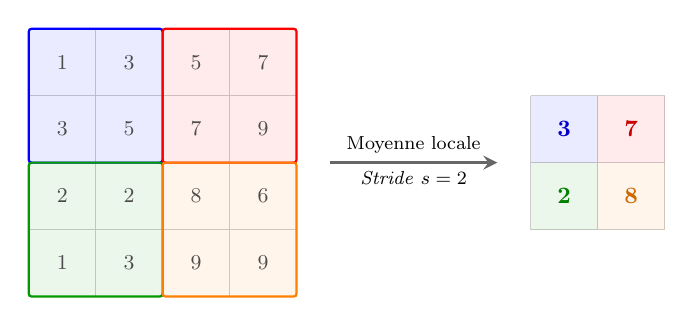
\begin{tikzpicture}[scale=0.85, transform shape]
        % --- GRILLE D'ENTREE (4x4) ---
        \draw[step=1cm, gray!40, thin] (0,0) grid (4,4);
        
        % Couleurs des blocs 2x2 (Style sobre et epure)
        \fill[blue, opacity=0.08] (0,2) rectangle (2,4);
        \fill[red, opacity=0.08] (2,2) rectangle (4,4);
        \fill[green!60!black, opacity=0.08] (0,0) rectangle (2,2);
        \fill[orange, opacity=0.08] (2,0) rectangle (4,2);

        % Cadres des blocs
        \draw[blue, thick, rounded corners=1pt] (0,2) rectangle (2,4);
        \draw[red, thick, rounded corners=1pt] (2,2) rectangle (4,4);
        \draw[green!60!black, thick, rounded corners=1pt] (0,0) rectangle (2,2);
        \draw[orange, thick, rounded corners=1pt] (2,0) rectangle (4,2);

        % Valeurs d'entree (Exemple numerique simple)
        \foreach \x/\y/\v in {0.5/3.5/1, 1.5/3.5/3, 0.5/2.5/3, 1.5/2.5/5,
                              2.5/3.5/5, 3.5/3.5/7, 2.5/2.5/7, 3.5/2.5/9,
                              0.5/1.5/2, 1.5/1.5/2, 0.5/0.5/1, 1.5/0.5/3,
                              2.5/1.5/8, 3.5/1.5/6, 2.5/0.5/9, 3.5/0.5/9} {
            \node[font=\small, text=black!70] at (\x, \y) {\v};
        }

        % --- FLECHE DE TRANSITION ---
        \draw[->, >=stealth, very thick, black!60] (4.5, 2) -- node[above, font=\footnotesize, text=black] {Moyenne locale} node[below, font=\footnotesize, text=black] {\textit{Stride} $s=2$} (7, 2);

        % --- GRILLE DE SORTIE (2x2) ---
        \begin{scope}[xshift=7.5cm, yshift=1cm]
            \draw[step=1cm, gray!40, thin] (0,0) grid (2,2);
            
            % Couleurs correspondantes
            \fill[blue, opacity=0.08] (0,1) rectangle (1,2);
            \fill[red, opacity=0.08] (1,1) rectangle (2,2);
            \fill[green!60!black, opacity=0.08] (0,0) rectangle (1,1);
            \fill[orange, opacity=0.08] (1,0) rectangle (2,1);

            % Valeurs calculees (moyennes)
            \node[font=\bfseries, text=blue!80!black] at (0.5, 1.5) {3};
            \node[font=\bfseries, text=red!80!black] at (1.5, 1.5) {7};
            \node[font=\bfseries, text=green!50!black] at (0.5, 0.5) {2};
            \node[font=\bfseries, text=orange!80!black] at (1.5, 0.5) {8};
        \end{scope}

    \end{tikzpicture}
    \caption{Illustration spatiale de l'opération d'\textit{average pooling}. Chaque bloc de $2 \times 2$ pixels de l'image d'entrée est remplacé par sa moyenne arithmétique, réduisant ainsi la résolution spatiale par un facteur $s=2$.}
    \label{fig:avg_pooling_spatial}
\end{figure}

\section{Rappel sur la SVD et les directions d'amplification}
\label{app:svd-sensibilite}

Soit
\[
    M \in \mathbb{C}^{m_{\mathrm{out}}N^2 \times m_{\mathrm{in}}N^2}
\]
la matrice représentant un opérateur de convolution multi-canaux. Comme cette matrice n'est pas
nécessairement carrée, on utilise la décomposition en valeurs singulières plutôt qu'une diagonalisation
classique par valeurs propres.

La décomposition en valeurs singulières de $M$ s'écrit
\[
    M = U \Sigma V^H,
\]
où $U$ et $V$ sont des matrices unitaires, et où $\Sigma$ est une matrice diagonale rectangulaire
contenant les valeurs singulières de $M$ :
\[
    \sigma_1 \geq \sigma_2 \geq \cdots \geq 0.
\]
Les colonnes de $V$ sont appelées vecteurs singuliers droits de $M$ : elles vivent dans l'espace
d'entrée. Les colonnes de $U$ sont appelées vecteurs singuliers gauches de $M$ : elles vivent dans
l'espace de sortie.

Pour comprendre pourquoi les vecteurs singuliers droits décrivent les directions d'amplification,
on considère la matrice auto-adjointe positive $M^H M$. À partir de la SVD, on obtient
\[
    M^H M
    =
    (U\Sigma V^H)^H(U\Sigma V^H).
\]
En utilisant $(ABC)^H = C^H B^H A^H$, il vient
\[
    M^H M
    =
    V\Sigma^H U^H U \Sigma V^H.
\]
Comme $U$ est unitaire, on a $U^H U = I$, donc
\[
    M^H M
    =
    V\Sigma^H \Sigma V^H.
\]
La matrice $\Sigma^H\Sigma$ est diagonale et contient les carrés des valeurs singulières :
\[
    \Sigma^H\Sigma
    =
    \operatorname{diag}(\sigma_1^2,\sigma_2^2,\dots).
\]
Ainsi,
\[
    M^H M
    =
    V
    \operatorname{diag}(\sigma_1^2,\sigma_2^2,\dots)
    V^H.
\]
Cela montre que les vecteurs singuliers droits de $M$ sont exactement les vecteurs propres de
$M^H M$, et que les valeurs propres associées sont les carrés des valeurs singulières.

En particulier, si $v_i$ désigne la $i$-ème colonne de $V$, alors
\[
    M^H M v_i
    =
    V D V^H v_i
    =
    V D e_i
    =
    V(\sigma_i^2 e_i)
    =
    \sigma_i^2 v_i,
\]
où
\[
    D=\operatorname{diag}(\sigma_1^2,\sigma_2^2,\dots).
\]
Ainsi,
\[
    M^H M v_i = \sigma_i^2 v_i.
\]

De manière équivalente, la valeur singulière $\sigma_i$ mesure l'amplification induite par $M$
dans la direction $v_i$. En effet,
\[
    \|Mv_i\|_2^2
    =
    (Mv_i)^H(Mv_i)
    =
    v_i^H M^H M v_i
    =
    v_i^H(\sigma_i^2 v_i)
    =
    \sigma_i^2 \|v_i\|_2^2.
\]
Comme $V$ est unitaire, ses colonnes forment une base orthonormée. En particulier,
\[
    \|v_i\|_2 = 1.
\]
On obtient donc
\[
    \|Mv_i\|_2 = \sigma_i.
\]

La plus grande valeur singulière décrit l'amplification maximale de $M$ parmi les entrées de norme
$1$ :
\[
    \sigma_1
    =
    \max_{\|x\|_2=1}\|Mx\|_2.
\]
Si $\sigma_1$ est simple, la direction qui réalise cette amplification maximale est le vecteur singulier
droit $v_1$. Si $\sigma_1$ est multiple, il n'y a pas une seule direction maximale : toute direction
unitaire dans le sous-espace associé à $\sigma_1$ donne la même amplification.

Dans le cadre de l'analyse fréquentielle des convolutions, les directions de forte sensibilité du réseau
correspondent donc aux vecteurs singuliers droits associés aux grandes valeurs singulières.

\section{Spectre de Fourier moyen des images propres}
\label{annexe:spectres_moyens_cifar}

Cette annexe présente le spectre de Fourier moyen des images non perturbées de CIFAR-10 et CIFAR-100.
L'objectif n'est pas de mesurer directement la sensibilité du modèle, mais d'observer quelles fréquences
sont naturellement présentes dans les données d'entrée.

\begin{figure}[H]
    \centering
    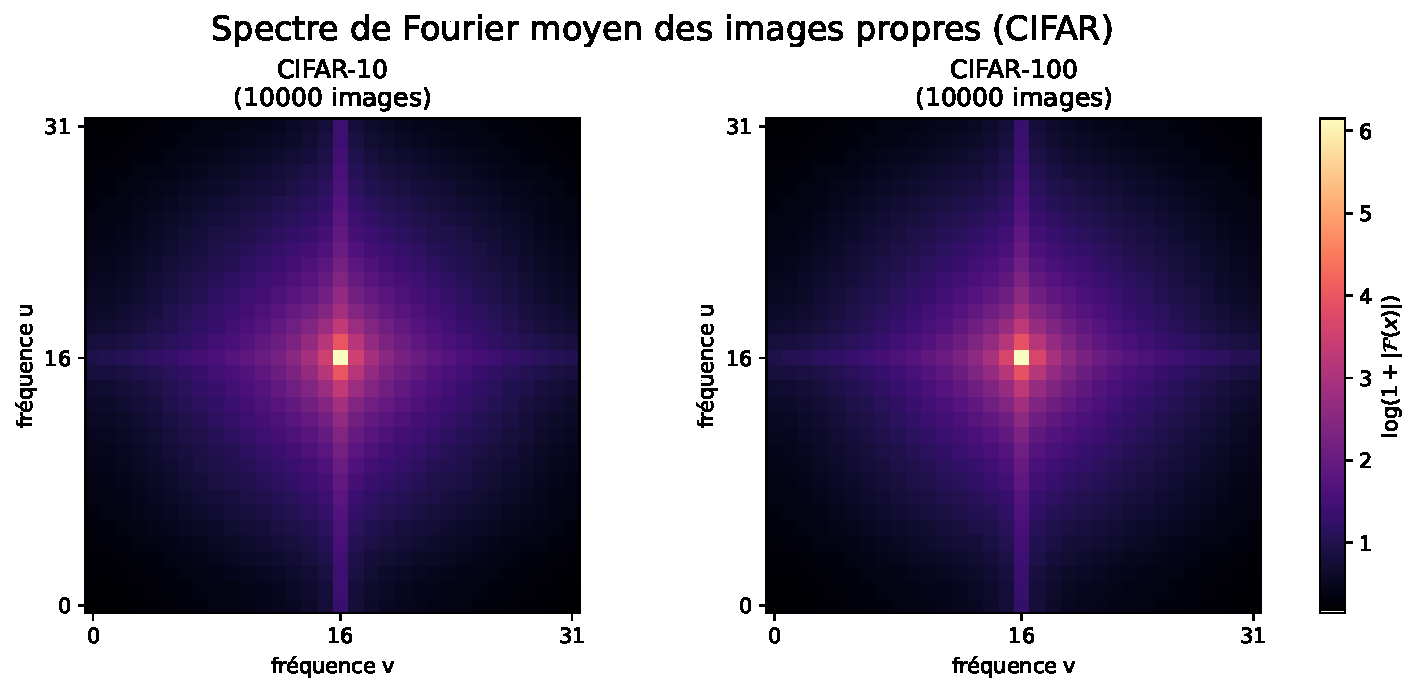
\includegraphics[width=\textwidth]{figures/results/mean_clean_spectrum_comparison_cifar.pdf}
    \caption{Spectre de Fourier moyen des images non perturbées de CIFAR-10 et CIFAR-100. Les valeurs affichées
    correspondent à $\log(1+|\mathcal{F}(x)|)$, moyennées sur les images du dataset.}
    \label{fig:mean_clean_spectrum_comparison_cifar}
\end{figure}

On observe que les deux datasets possèdent une structure fréquentielle très similaire : 
l'énergie est fortement concentrée autour du centre du spectre et décroît progressivement selon une forme 
proche d'un losange. Les lignes horizontale et verticale plus marquées indiquent également que certaines 
directions fréquentielles sont plus présentes que d'autres dans les images non perturbées.

Cette observation fournit une piste d'interprétation pour les heatmaps SFA. Elle montre que les images
d'entrée possèdent elles-mêmes une organisation fréquentielle non uniforme. La sensibilité du modèle
peut donc dépendre à la fois de l'architecture et des statistiques des données utilisées pendant
l'entraînement.

Cette comparaison reste toutefois descriptive. Le spectre moyen caractérise les images d'entrée, alors
que les heatmaps SFA mesurent la réponse du modèle à des perturbations imposées. Les deux objets ne
doivent donc pas être confondus.

\section{Analyse complémentaire : rôle du mélange des canaux dans la SFA}
\label{annexe:color_sfa}

Dans le cadre théorique présenté au chapitre précédent, les directions singulières d'un modèle
convolutionnel linéarisé peuvent s'écrire sous une forme du type
\[
    v = a \otimes q_{u,v},
\]
où \(q_{u,v}\) représente une composante spatiale de Fourier et où
\(a \in \mathbb{R}^3\) décrit le mélange entre les canaux rouge, vert et bleu.

La \textit{Single Fourier Attack} utilisée dans le protocole principal simplifie ce cadre. Elle ne cherche
pas à optimiser simultanément la fréquence spatiale et le vecteur couleur \(a\). Le même motif de
Fourier est appliqué aux trois canaux RGB, ce qui revient à utiliser le vecteur
\[
    a_{\mathrm{uni}} = (1,1,1).
\]
L'espace de recherche est donc réduit au choix de la fréquence $(u,v)$. Cette simplification
rend l'attaque beaucoup plus simple à évaluer, puisqu'il suffit de parcourir les fréquences du
domaine de Fourier. Elle est également cohérente avec la contrainte $\ell_\infty$ utilisée dans
le protocole principal : le motif est appliqué avec l'amplitude maximale autorisée sur chacun des
trois canaux.

Nous distinguons alors deux manières de contraindre le mélange entre canaux. La première
conserve une contrainte comparable à la SFA standard en norme $\ell_\infty$, afin de tester si
un autre choix de direction couleur peut améliorer l'attaque à amplitude maximale identique. La
seconde utilise un budget de type $\ell_1$ sur les coefficients du vecteur couleur. Dans ce cas,
un vecteur comme $a=(3,0,0)$ est possible : le budget total est concentré sur un seul canal, ce
qui ne correspond plus exactement à la contrainte de la SFA standard. Les deux variantes ne
mesurent donc pas exactement la même chose ; elles servent plutôt à tester si le choix du mélange
RGB peut renforcer l'effet d'une fréquence de Fourier.

\subsection*{Recherche de vecteurs RGB par fréquence}

La figure~\ref{fig:color_sfa_foolratio_and_activation_grids} compare la SFA standard avec des variantes
où le vecteur RGB \(a\) est choisi parmi un ensemble restreint de combinaisons possibles.

\begin{figure}[H]
    \centering
    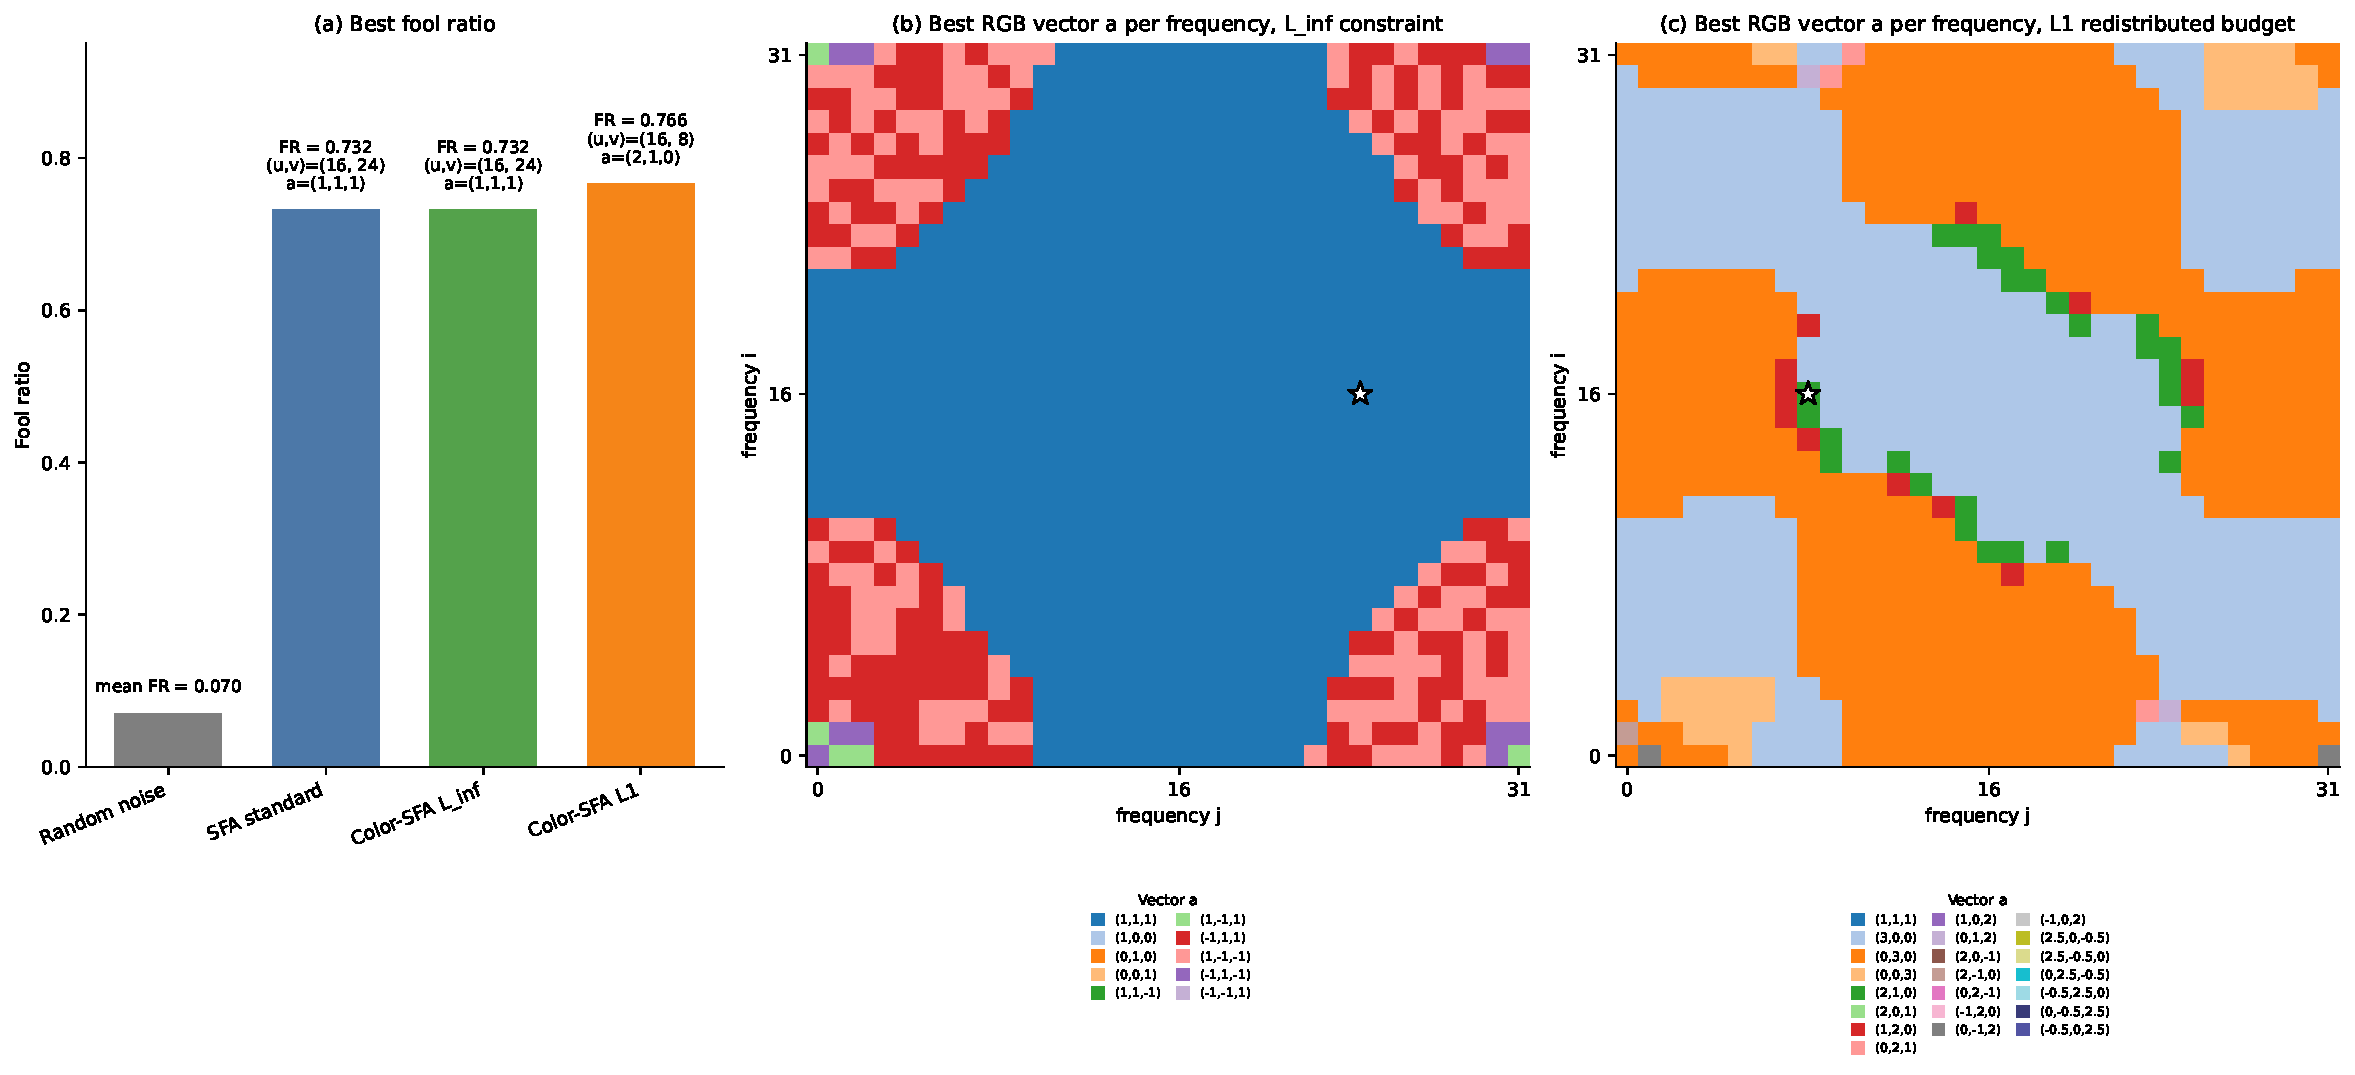
\includegraphics[width=\textwidth]{figures/results/color_sfa_foolratio_and_activation_grids.pdf}
    \caption{Comparaison entre la SFA standard et des variantes où le vecteur RGB \(a\) est choisi par fréquence.
    À gauche, le meilleur \textit{fool ratio} obtenu par chaque méthode est comparé à la baseline de bruit
    aléatoire. Au centre et à droite, chaque case indique le meilleur vecteur RGB trouvé pour la fréquence
    correspondante, selon deux contraintes de budget différentes.}
    \label{fig:color_sfa_foolratio_and_activation_grids}
\end{figure}

Dans la variante renormalisée en norme $\ell_\infty$, la meilleure variante colorée retrouve
pratiquement le même résultat que la SFA standard. Ce qui indique que, sous cette contrainte, le
choix d'un mélange RGB différent n'améliore pas significativement l'attaque par rapport à la
direction uniforme $(1,1,1)$.

Avec la variante sous budget $\ell_1$ sur les coefficients couleur, le meilleur score augmente légèrement,
passant d'environ \(0.732\) à \(0.766\), avec la fréquence \((16,8)\) et le vecteur \(a=(2,1,0)\).
Ce qui est assez modeste dans notre cas.

\subsection*{Comparaison de directions couleur fixes}

Nous avons ensuite comparé plusieurs directions couleur simples :
\[
(1,1,1), \quad (1,0,0), \quad (0,1,0), \quad (0,0,1),
\]
ainsi que des directions chromatiques opposées :
\[
(1,-1,0), \quad (1,0,-1), \quad (0,1,-1),
\]
et une direction de type luminance.

Les résultats de la figure~\ref{fig:color_sfa_cifar10} montrent que la direction standard
$(1,1,1)$ reste nettement la plus efficace. Les directions appliquées à un seul canal ont un effet
plus faible, tandis que les directions chromatiques opposées $(1,-1,0)$, $(1,0,-1)$ et
$(0,1,-1)$ donnent des fool ratios presque nuls.

\begin{figure}[H]
    \centering
    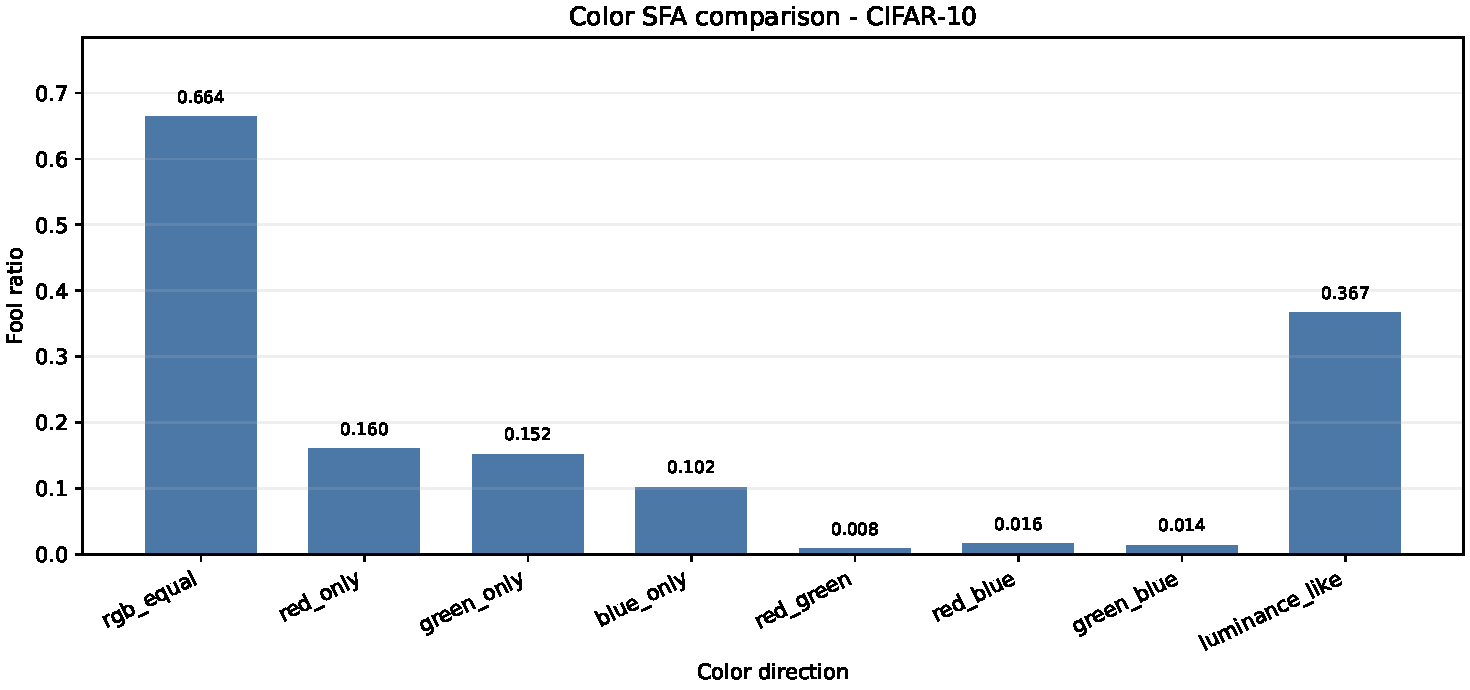
\includegraphics[width=0.85\textwidth]{figures/results/color_sfa_cifar10_barplot.pdf}
    \caption{Comparaison de plusieurs directions couleur pour la \textit{Single Fourier Attack}
    sur CIFAR-10.}
    \label{fig:color_sfa_cifar10}
\end{figure}

Cette observation suggère que, pour la fréquence étudiée, les directions chromatiques opposées
sont faiblement transmises par le réseau. Nous pouvons l'interpréter à partir du cadre
multi-canaux. Pour une fréquence fixée $(u,v)$, l'effet d'une direction couleur
$a \in \mathbb{R}^3$ est décrit par la matrice de mélange $G^{(u,v)}$ :
\[
    \beta = G^{(u,v)}a.
\]
La SFA standard correspond au choix
\[
    a_{\mathrm{uni}} = (1,1,1),
\]
c'est-à-dire à une variation commune des trois canaux RGB.

\paragraph{Cas idéalement symétrique.}
Supposons que, pour la fréquence considérée, le réseau réponde de la même manière aux trois
canaux d'entrée. Cela revient à supposer que les trois colonnes de $G^{(u,v)}$ sont identiques :
\[
    G^{(u,v)}
    =
    \begin{pmatrix}
    | & | & | \\
    g & g & g \\
    | & | & |
    \end{pmatrix}
    =
    g
    \begin{pmatrix}
    1 & 1 & 1
    \end{pmatrix},
\]
où $g \in \mathbb{C}^{m_{\mathrm{out}}}$ décrit la réponse fréquentielle commune du réseau.

Alors, pour toute direction couleur $a=(a_R,a_G,a_B)$, on obtient
\[
    G^{(u,v)}a
    =
    g(a_R+a_G+a_B).
\]
L'amplification dépend donc uniquement de la somme des composantes de $a$. Sous une contrainte
$\ell_\infty$ comparable à celle de la SFA standard,
\[
    |a_R|, |a_G|, |a_B| \leq 1,
\]
cette somme est maximale en valeur absolue pour
\[
    a=(1,1,1)
\]
ou pour son opposé. Ainsi, dans ce cadre symétrique simplifié, la direction uniforme
$a_{\mathrm{uni}}$ est optimale.

Inversement, toute direction couleur vérifiant
\[
    a_R+a_G+a_B=0
\]
est annulée par $G^{(u,v)}$. C'est le cas des directions chromatiques opposées
\[
    (1,-1,0), \qquad (1,0,-1), \qquad (0,1,-1).
\]
Dans ce modèle simplifié, ces directions appartiennent donc au noyau de la matrice de mélange
fréquentielle :
\[
    G^{(u,v)}a = 0.
\]

\paragraph{Cas approximativement symétrique.}
Dans un réseau réel, les colonnes de $G^{(u,v)}$ ne sont pas exactement identiques. On peut
cependant séparer une composante commune aux trois canaux et un terme résiduel :
\[
    G^{(u,v)}
    =
    g
    \begin{pmatrix}
    1 & 1 & 1
    \end{pmatrix}
    + E,
\]
où l'on peut prendre
\[
    g
    =
    \frac{1}{3}G^{(u,v)}
    \begin{pmatrix}
    1 \\ 1 \\ 1
    \end{pmatrix}.
\]
Le terme $E$ mesure alors l'écart à une réponse parfaitement commune aux trois canaux.

Pour une direction chromatique opposée telle que $a_R+a_G+a_B=0$, la composante commune
disparaît :
\[
    G^{(u,v)}a = Ea.
\]
Ainsi, si $\|E\|$ est faible, alors
\[
    \|G^{(u,v)}a\|_2
    \leq
    \|E\|\,\|a\|_2.
\]
Les directions chromatiques opposées ne sont donc plus annulées exactement, mais elles restent
faiblement transmises lorsque le mélange fréquentiel entre les canaux est proche d'une réponse
commune.

Cette proposition fournit une interprétation théorique des résultats observés dans la
figure~\ref{fig:color_sfa_cifar10}. La forte efficacité de $(1,1,1)$ suggère que la fréquence
étudiée active principalement une direction commune aux canaux, tandis que les faibles scores
des directions chromatiques opposées peuvent s'expliquer par une quasi-annulation dans le
mélange fréquentiel des canaux.

\section{Heatmaps internes par couche}
\label{annexe:heatmaps_internes_couches}

En complément de l'analyse d'amplification présentée dans le chapitre principal, nous visualisons ici
l'effet des perturbations de Fourier à différents niveaux internes du réseau. Pour chaque fréquence,
nous mesurons la variation moyenne normalisée des activations après perturbation, puis nous la
comparons au \textit{fool ratio} final.

\begin{figure}[H]
    \centering
    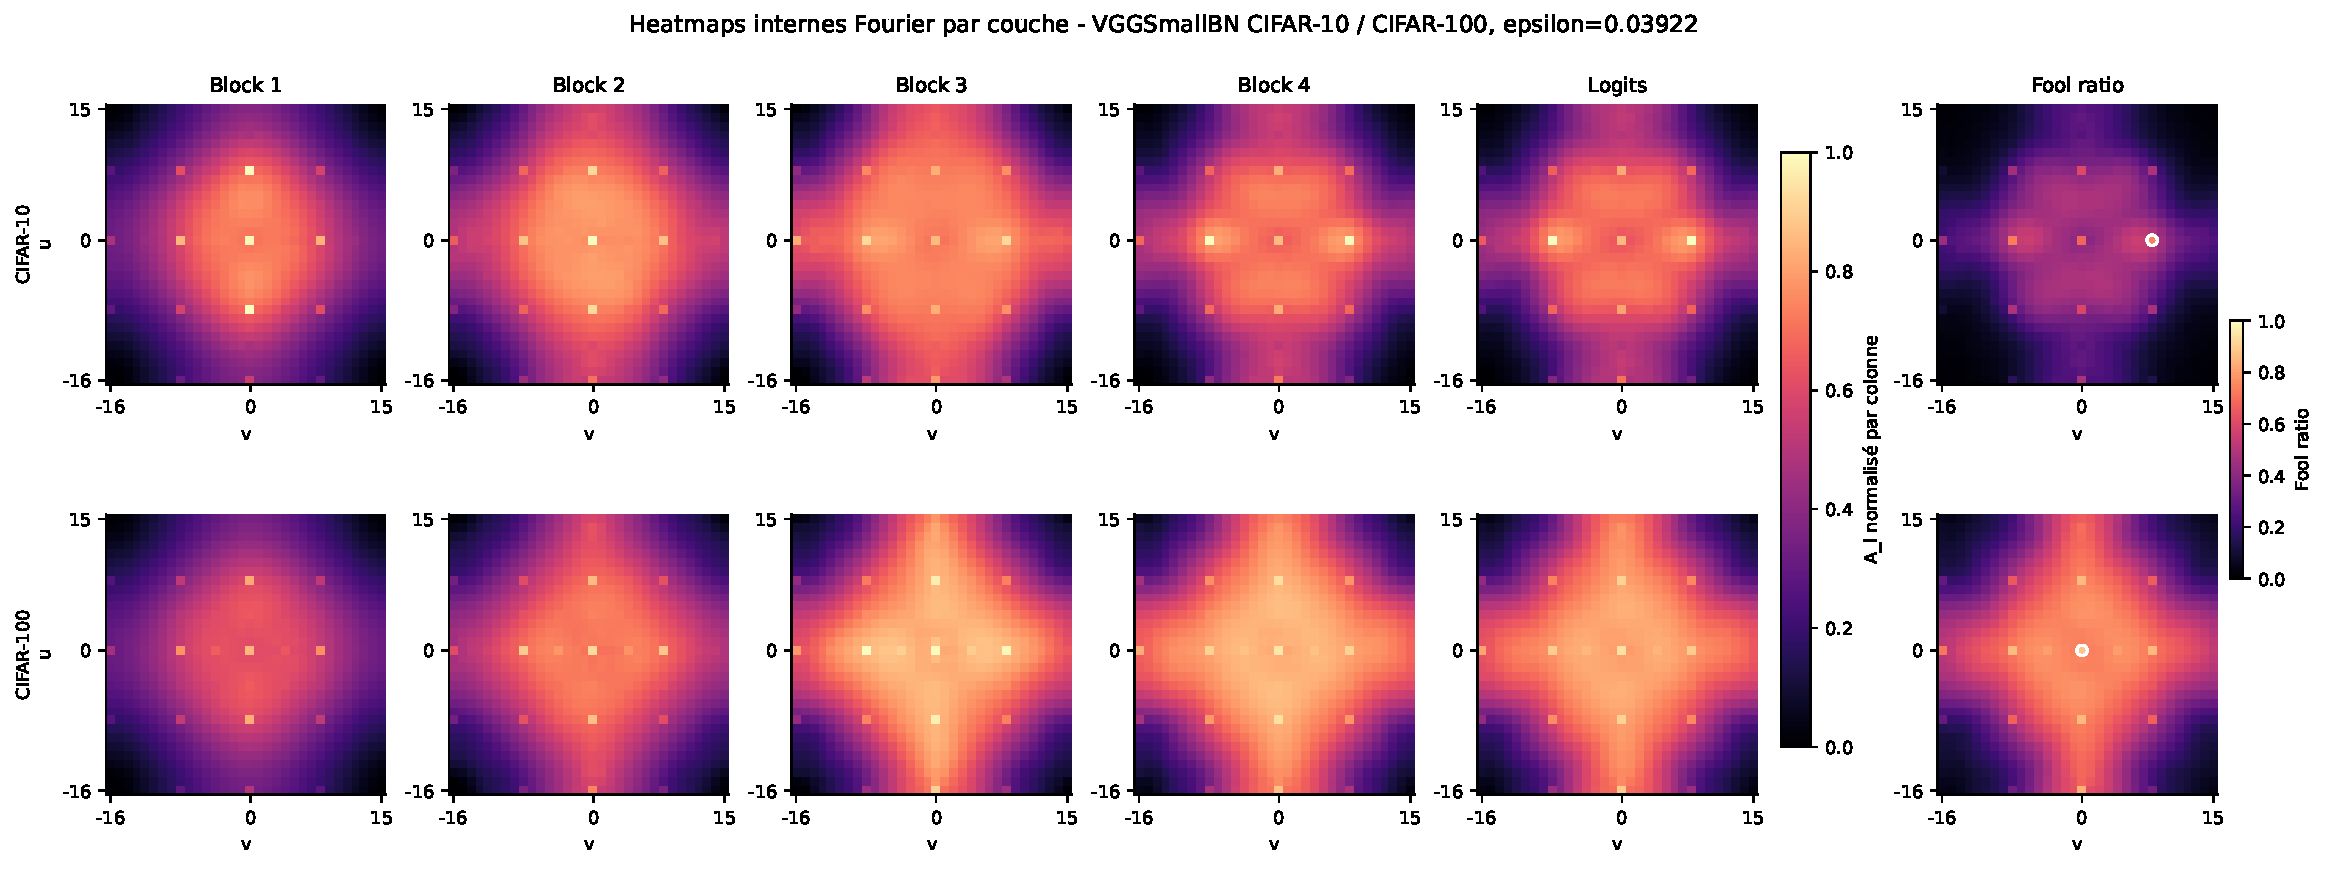
\includegraphics[width=\textwidth]{figures/results/layerwise_fourier_heatmaps_comparison_vgg_cifar10_cifar100.pdf}
    \caption{Heatmaps internes par couche pour \texttt{VGGSmallBN} sur CIFAR-10 et CIFAR-100.
    Les premières colonnes représentent la variation moyenne normalisée des activations internes après
    perturbation de Fourier. La dernière colonne indique le \textit{fool ratio} final.}
    \label{fig:annexe_layerwise_fourier_heatmaps}
\end{figure}

Ces visualisations montrent que la structure fréquentielle observée dans les heatmaps finales apparaît
déjà dans les représentations internes du réseau. Elle devient plus marquée dans les blocs profonds et
dans les logits, ce qui suggère que certaines fréquences sont progressivement amplifiées au cours du
traitement convolutionnel.

\section{Analyse complémentaire des marges logits et des frontières locales}
\label{annexe:marges-logits}

Cette annexe complète l'analyse expérimentale du chapitre~4. L'objectif est de mieux comprendre
pourquoi le modèle entraîné sur CIFAR-100 apparaît plus fragile que celui entraîné sur CIFAR-10.

\subsection{Distribution des marges logits}

Pour chaque image du jeu de test, on calcule les logits produits par le modèle. On note ensuite
$z_{(1)}$ le plus grand logit et $z_{(2)}$ le deuxième plus grand logit. La marge logit est définie par
\[
    m(x) = z_{(1)}(x) - z_{(2)}(x).
\]

Cette quantité mesure basiquement l'écart entre la classe prédite et la classe concurrente la plus proche selon
le modèle.

La figure~\ref{fig:logit-margin-histograms} compare les distributions des marges logits pour
VGGSmallBN sur CIFAR-10 et CIFAR-100. On observe que la distribution de CIFAR-100 est
nettement plus concentrée vers les faibles marges. La médiane est d'environ $4.15$ pour CIFAR-100,
contre environ $11.12$ pour CIFAR-10. Cela signifie que, sur CIFAR-100, les prédictions du modèle
sont en moyenne moins fortement séparées de leur seconde meilleure classe.

\begin{figure}[H]
    \centering
    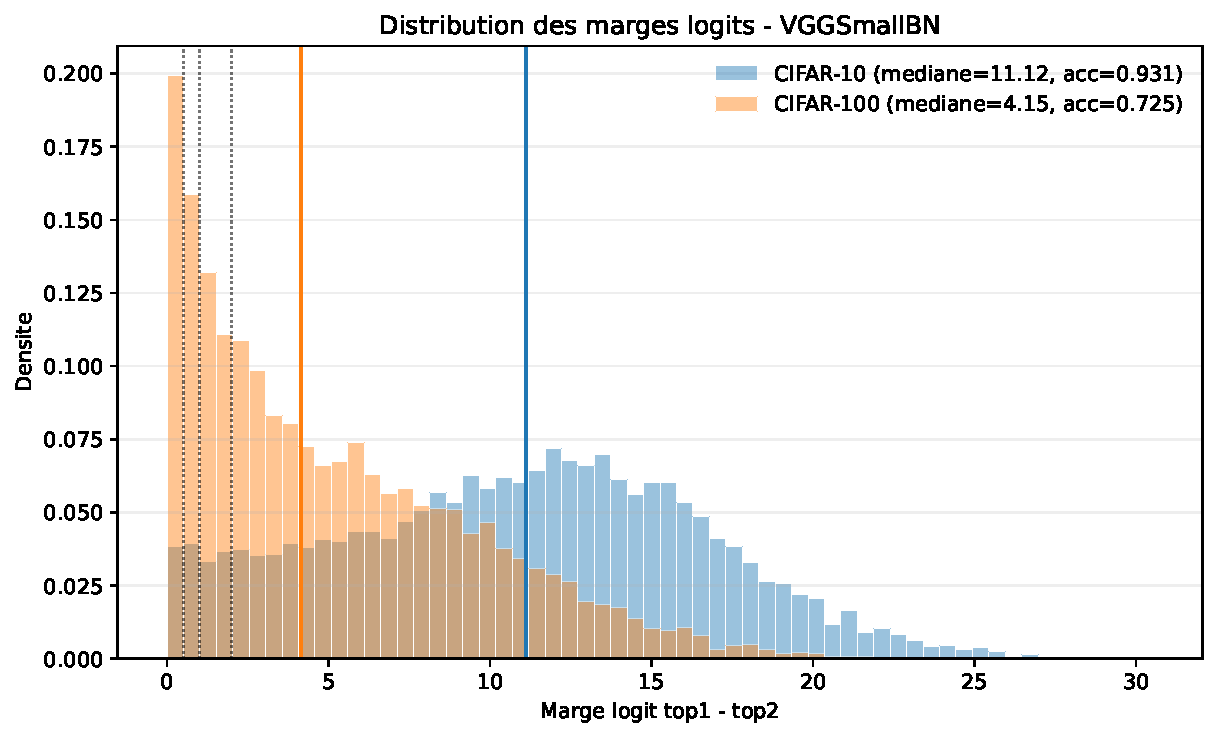
\includegraphics[width=0.85\textwidth]{figures/results/logit_margin_histograms_cifar10_cifar100.pdf}
    \caption{Distribution des marges logits pour VGGSmallBN sur CIFAR-10 et CIFAR-100. La marge est définie comme la différence entre le plus grand logit et le deuxième plus grand logit.}
    \label{fig:logit-margin-histograms}
\end{figure}

Ce résultat donne un appui supplémentaire à l'interprétation proposée dans le chapitre~4 :
la plus grande fragilité observée sur CIFAR-100 ne vient pas seulement du choix d'une fréquence
particulière, mais aussi du fait que les décisions du modèle semblent moins séparées. 

% \subsection{Carte moyenne de stabilité locale}

% En complément de l'analyse des marges logits, nous construisons une carte moyenne de stabilité
% locale autour des images correctement classées. L'objectif est de visualiser, dans une coupe
% bidimensionnelle de l'espace d'entrée, dans quelle mesure les prédictions restent stables lorsque
% l'on perturbe les images selon deux directions fréquentielles sensibles.

% Pour une image $x$, on considère les perturbations de la forme
% \[
%     x_{\alpha,\beta}
%     =
%     x + \alpha d_1 + \beta d_2,
% \]
% où $d_1$ correspond à la direction SFA principale du dataset, et $d_2$ à une seconde direction
% fréquentielle sensible.

% Pour chaque point $(\alpha,\beta)$ de la grille, nous calculons la proportion d'images pour
% lesquelles la prédiction reste identique à celle de l'image propre :
% \[
%     P_{\mathrm{same}}(\alpha,\beta)
%     =
%     \frac{1}{M}
%     \sum_{k=1}^{M}
%     \mathbf{1}\left[
%         f(x_k+\alpha d_1+\beta d_2)=f(x_k)
%     \right].
% \]
% Cette quantité vaut $1$ lorsque toutes les images gardent la même prédiction, et $0$ lorsque
% toutes les prédictions changent. Elle fournit donc une mesure moyenne de la stabilité locale du
% modèle dans la coupe considérée.

% Les cartes sont calculées sur $500$ images correctement classées par dataset, avec une grille
% de taille $41\times 41$.

% \begin{figure}[H]
%     \centering
%     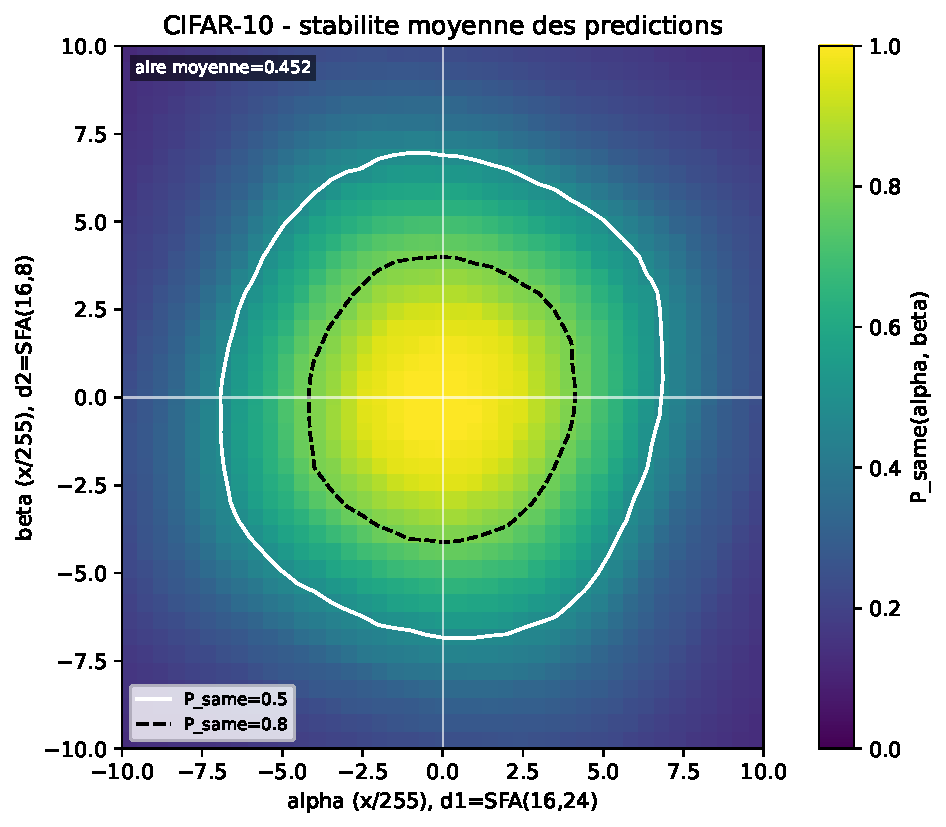
\includegraphics[width=0.48\textwidth]{figures/results/average_decision_boundary_cifar10.pdf}
%     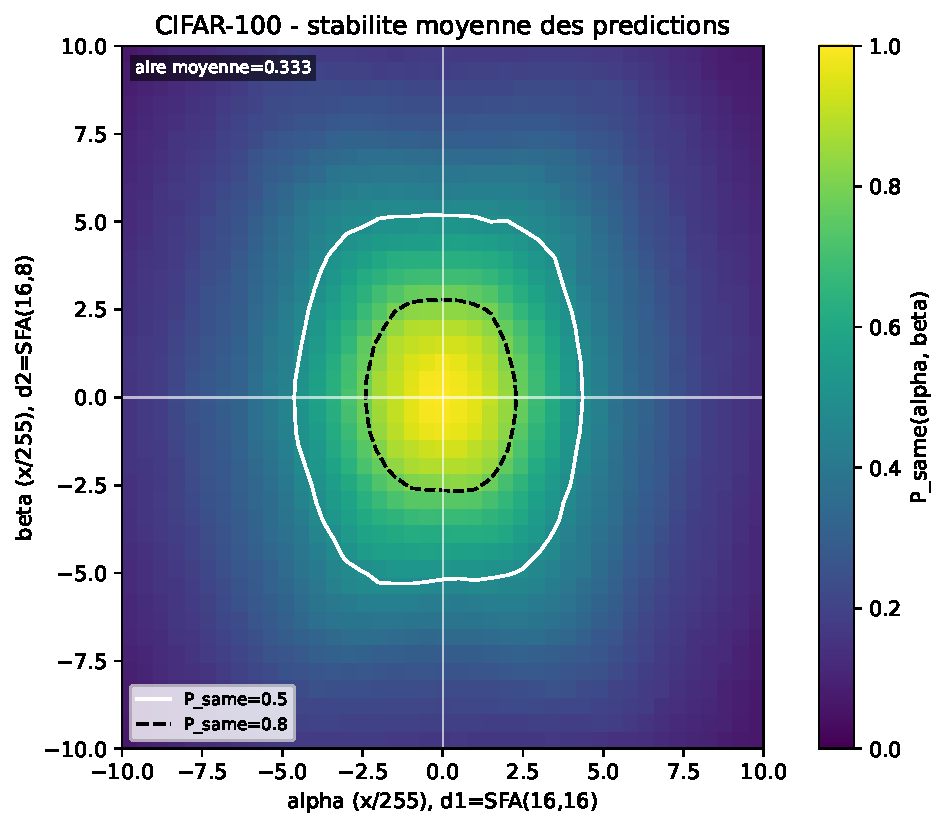
\includegraphics[width=0.48\textwidth]{figures/results/average_decision_boundary_cifar100.pdf}
%     \caption{Cartes moyennes de stabilité locale pour VGGSmallBN sur CIFAR-10 et CIFAR-100. Chaque point indique la proportion d'images dont la prédiction reste inchangée après perturbation selon deux directions fréquentielles sensibles.}
%     \label{fig:average-decision-boundary}
% \end{figure}

% \begin{table}[H]
%     \centering
%     \begin{tabular}{lcccc}
%         \toprule
%         Dataset & Aire stable moyenne & Largeur $P_{\mathrm{same}}\geq 0.5$ & Largeur $P_{\mathrm{same}}\geq 0.8$ & $\alpha$ critique moyen \\
%         \midrule
%         CIFAR-10  & 0.4518 & $13.00/255$ & $8.00/255$ & $5.81/255$ \\
%         CIFAR-100 & 0.3330 & $8.50/255$  & $4.00/255$ & $4.46/255$ \\
%         \bottomrule
%     \end{tabular}
%     \caption{ Les largeurs sont mesurées sur la ligne $\beta=0$, avec Les coefficients $\alpha$ et 
%     $\beta$ qui varient dans l'intervalle $[-10/255,10/255]$}
%     \label{tab:average-decision-boundary}
% \end{table}

% Les résultats du tableau~\ref{tab:average-decision-boundary} montrent que la région moyenne de
% stabilité est plus réduite sur CIFAR-100 que sur CIFAR-10. L'aire stable moyenne passe de
% $0.4518$ à $0.3330$, et la largeur de la région stable le long de la direction SFA diminue également.
% Pour le seuil $P_{\mathrm{same}}\geq 0.8$, cette largeur est divisée par deux, passant de $8.00/255$
% sur CIFAR-10 à $4.00/255$ sur CIFAR-100.

% Cette observation est cohérente avec les résultats principaux du chapitre~4 : le modèle entraîné
% sur CIFAR-100 est globalement plus sensible aux perturbations fréquentielles. Elle complète
% également l'analyse des marges logits, en montrant que cette fragilité se manifeste aussi dans
% une coupe locale de l'espace d'entrée.

% Il faut toutefois rester prudent dans l'interprétation. Ces cartes ne représentent pas la frontière
% de décision complète du réseau, qui vit dans un espace de dimension $32\times32\times3$.
% Elles décrivent seulement une coupe bidimensionnelle construite à partir de deux directions
% fréquentielles sensibles. Elles doivent donc être lues comme une visualisation complémentaire,
% et non comme une preuve complète de la géométrie globale des frontières de décision.